%
% To start the document, use
%  \levela{...}
% For lover level, sections use
%  \levelb{...}
%  \levelc{...}
%
\levela{The ARTS concept}
 \label{sec:concept}

%
% Document history, format:
%  \starthistory
%    date1 & text .... \\
%    date2 & text .... \\
%    ....
%  \stophistory
%
\starthistory
  000616 & Created by Stefan Buehler, based on my DPG2000 poster.
\stophistory

%
% Symbol table, format:
%  \startsymbols
%    ... & \verb|...| & text ... \\
%    ... & \verb|...| & text ... \\
%    ....
%  \stopsymbols
%
%

%
% Introduction
%
This section describes the basic ideas underlying ARTS. It also
introduces some terminology. You should read it if you want
to understand how the program works and how it can be used
efficiently.

\levelb{Introduction}
%====================
\label{sec:concept:intro}

The number of satellite sensors in the millimeter and sub-millimeter
spectral range is rapidly growing. They use various frequency
bands and observation geometries. Two important groups of
sensors are for example the nadir viewing millimeter wave
sensors like AMSU\footnote{The \textbf{A}dvanced
  \textbf{M}icrowave \textbf{S}ounding \textbf{U}nit is a
  sensor on board the polar orbiting satellites of the
  US-American National Aeronautics and Space Administration.}
and the limb viewing sub-millimeter wave sensors like the
planned SMILES\footnote{The \textbf{S}uperconducting
  Sub-\textbf{Mi}llimeter Wave \textbf{L}imb \textbf{E}mission
  \textbf{S}ounder is a Japanese Sensor which will be flown
  for the first time on the International Space Station.}.

For the data analysis all such sensors require accurate and
fast forward models, which can simulate measurements for a
given atmospheric (and maybe ground) state. Depending on the
objective of the sensor, the measurement will depend for
example on the distribution of atmospheric temperature, water
vapor, ozone, and many other trace gases.

So far, a lot of effort has been wasted in developing
dedicated forward models for different sensors, although all
these models have many features in common. Moreover, existing
models were not easily modifiable and extendable. Hence, it
was decided to develop a new model which emphasizes
modularity, extendibility, and generality.


\levelb{Enter: ARTS}
%===================
\label{sec:concept:arts}

The most important notion in ARTS is the \emph{workspace}. All
physical quantities (for example absorption coefficients) are
\emph{workspace variables}. But workspace variables can also be of
a more technical nature, for example various grids. 

The program performs a calculation by executing a list of
\emph{workspace methods}, which are specified in a
controlfile. These workspace methods take workspace variables as
input, and generate workspace variables as output. Additional
input parameters can be specified as \emph{keyword parameters} in
the controlfile (Figure \ref{fig:method}).

\begin{figure}
  \begin{center}
    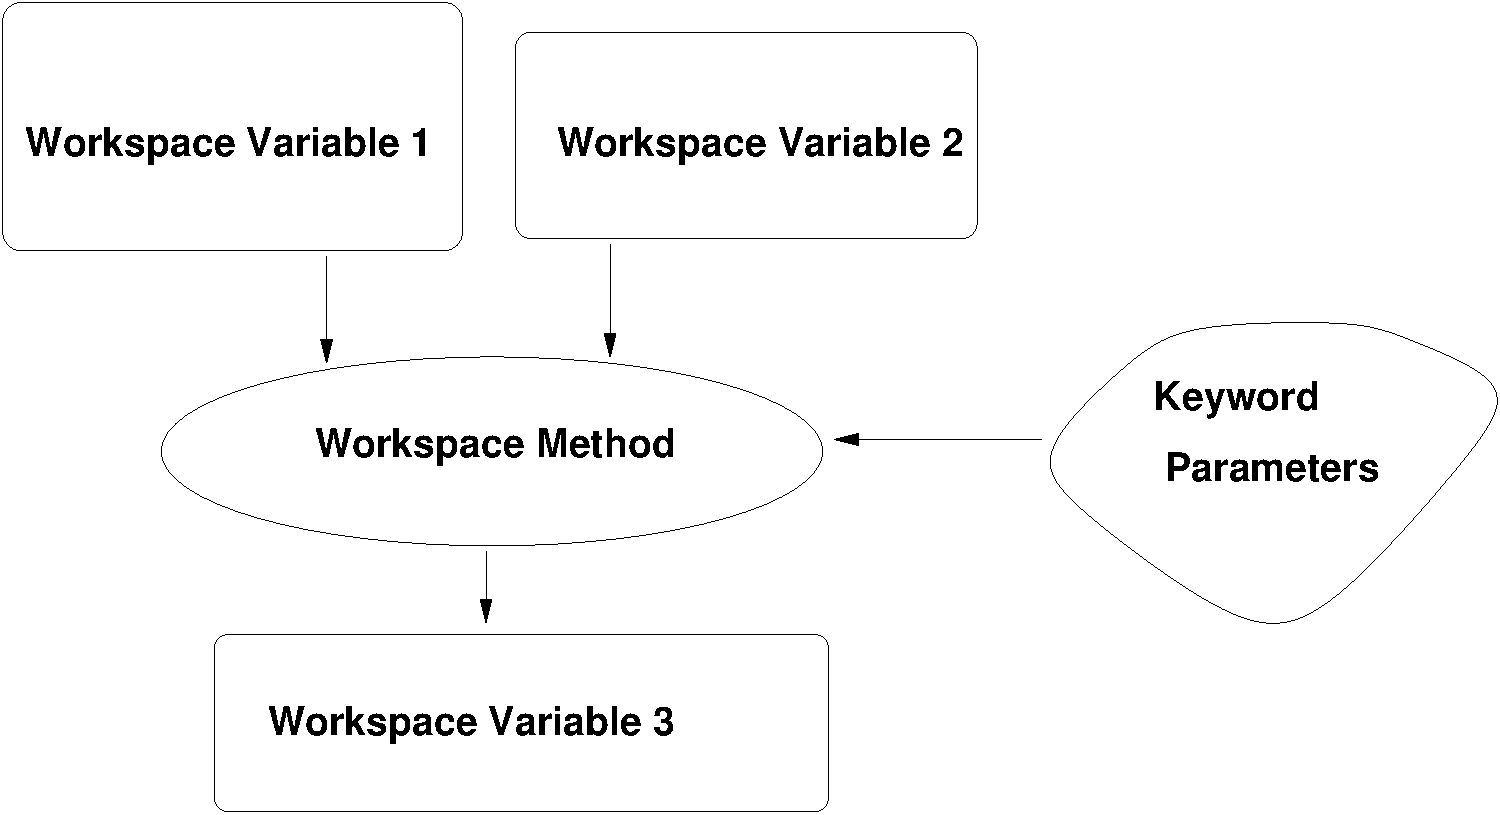
\includegraphics[width=\hsize,draft=false]{method}
    \caption{\emph{Specific}
        workspace methods act on specific workspace variables to
        generate other specific workspace variables. Additional input
        parameters can be specified as keyword parameters in the
        controlfile.}
    \label{fig:method}
  \end{center}
\end{figure}

It is important to note that the controlfile has a fixed and
well-defined syntax. This syntax is understood by the ARTS parser.
The great advantage of this concept is that it is very easy to add
new workspace variables and new workspace methods. The program has
an internal lookup table which lists all workspace methods, as well
as their input variables, output variables, and keyword
parameters. To add a new method, one just has to add an entry to
this lookup table, and write the code for the method itself. No
further changes to the program are necessary. In particular, no
changes to the program logic or to the parser. How such an extension
can be made practically is described in Section \ref{sec:development}.


\levelb{Generic Workspace Methods}
%=================================
\label{sec:concept:generic}

Generic methods (Figure \ref{fig:generic_method}) allow the user of the
program even more freedom than specific methods. A generic method is
for example \verb|VectorReadAscii|, which can be used to read any
workspace variable which is a vector from an ASCII file. For example
\begin{quote}
  \verb|VectorReadAscii(f_mono){"freqeuency_grid.dat"}|
\end{quote}
will read the specified file and generate the workspace variable
\verb|f_grid|.

\begin{figure}
  \begin{center}
    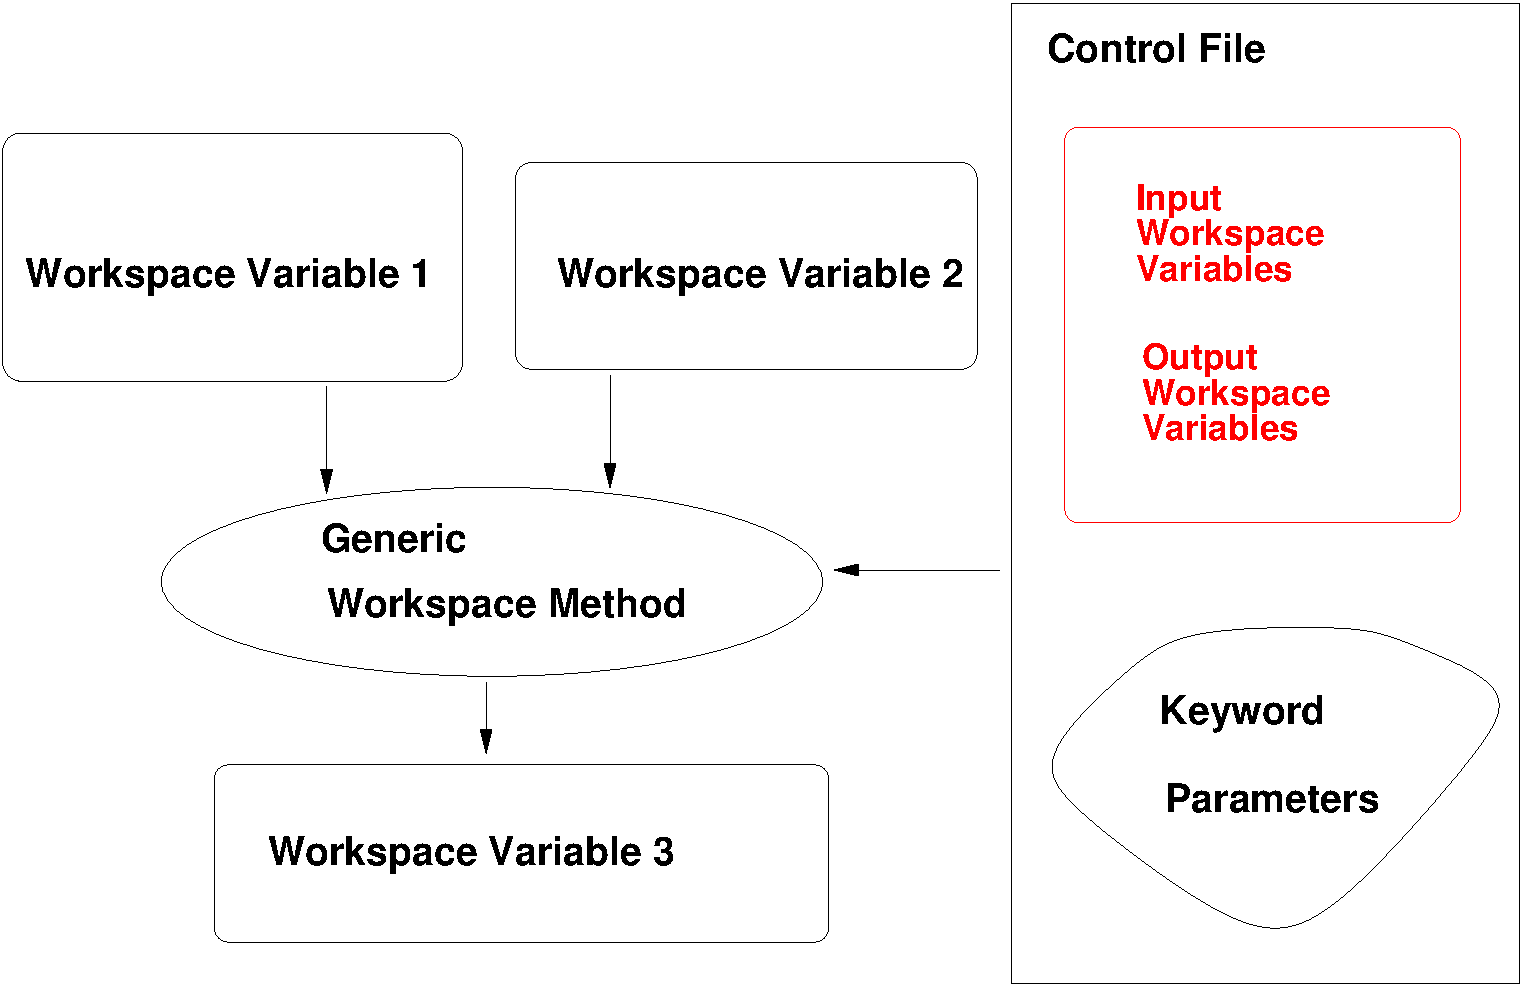
\includegraphics[width=\hsize,draft=false]{generic_method}
    \caption{For \emph{generic}
      workspace methods the workspace variables to act on are
        specified in the controlfile.}
    \label{fig:generic_method}
  \end{center}
\end{figure}

Generic methods are particularly useful for IO operations like in the
example above. No new IO functions are necessary for new workspace
variables, as long as they are of standard types already known to the
program (for example vectors or matrices).  Section
\ref{sec:concept:example} gives a short example of a controlfile which
illustrates the use of both generic and specific methods.

\levelb{An example controlfile}
%=================================
\label{sec:concept:example}

\begin{verbatim}
# An example ARTS controlfile that calculates absorption
# coefficients. 
# SAB 16.06.2000

# --------------------< A specific method >--------------------
#                      -------------------
# Read the spectroscopic line data from the HITRAN catalogue and
# create the workspace variable `lines':
linesReadFromHitran {
   filename = "../../data/spectroscopy/hitran96/hitran96_h2o.par"
   fmin     = 0
   fmax     = 1000e12 
}

# Optionally write the line list to a file:
linesWriteToFile{""} 

 
# This defines the list of tag groups (`tag_groups'). Absorption
# coefficients will be calculated separately for each tag group. This
# is necessary in order to calculate weighting functions later on.
# The lines are assigned to the tag groups in the order as the groups
# are specified here. That means the last group H2O gets assigned all
# the H2O lines that do not fit in any other group.
tag_groupsDefine{
      [ "H2O-161",
        "H2O-181",
        "H2O-171",
        "H2O" ] 
}

# This separates the lines into the different tag groups and creates
# the workspace variable `lines_per_tg':
lines_per_tgCreateFromLines{}

lines_per_tgWriteToFile{""} 


# --------------------< A generic method >--------------------
#                      ------------------
# Read the pressure, temperature, and altitude profiles and create 
# the workspace variable `raw_ptz_1d':
MatrixReadFromFile (raw_ptz_1d) 
        {"../../data/atmosphere/fascod/midlatitude-summer.tz.am"}

# The same for the input VMR profiles:
raw_vmrs_1dReadFromScenario
        {"../../data/atmosphere/fascod/midlatitude-summer"}

# Optionally write this to a file:
ArrayOfMatrixWriteToFile (raw_vmrs_1d) {""}


# Create the pressure grid `p_abs':
VectorLinSpace(p_abs){
        start = 1000
        stop  = 1
        step  = -1 
}

VectorWriteToFile(p_abs){""}


# Now interpolate all the raw atmospheric input onto the pressure 
# grid and create the atmospheric variables `t_abs', `z_abs', `vmrs'
AtmFromRaw1D{}

# Optionally write these to files:
VectorWriteToFile (t_abs) {""}
VectorWriteToFile (z_abs) {""}
ArrayOfVectorWriteToFile (vmrs)  {""}


# Create the frequency grid `f_abs':
VectorLinSpace(f_abs){
        start = 1
        stop  = 1000
        step  = 1    
}


# Calculate absorption coefficients, both total (`abs') and 
# separately for each tag group (`abs_per_tg'):
absCalc{}

# These we definitely want to write to files!
MatrixWriteToFile (abs) {""}
ArrayOfMatrixWriteToFile (abs_per_tg) {""}
\end{verbatim}


%%% Local Variables: 
%%% mode: latex
%%% TeX-master: "main"
%%% End: 
